\subsection{Lab18: Esquema de la Modulación y Demodulación DPSK en GNU Radio}
%*********************
\begin{frame}{}

\pgfdeclareimage[width=\paperwidth,height=\paperheight]{bg}{imagenes/fondo_lab}
\setbeamertemplate{background}{\pgfuseimage{bg}}

\bfseries{\textrm{ \Large Lab 18: \\Esquema de la Modulación y \\Demodulación DPSK \\en GNU Radio}}
\raggedright
\end{frame}
%********************

\begin{frame}{Esquema de la Modulación y Demodulación DPSK en GNU Radio}

\pgfdeclareimage[width=\paperwidth,height=\paperheight]{bg}{imagenes/fondo3}
\setbeamertemplate{background}{\pgfuseimage{bg}}

\begin{figure}[H]
	\vspace{-3mm}
	\centering
	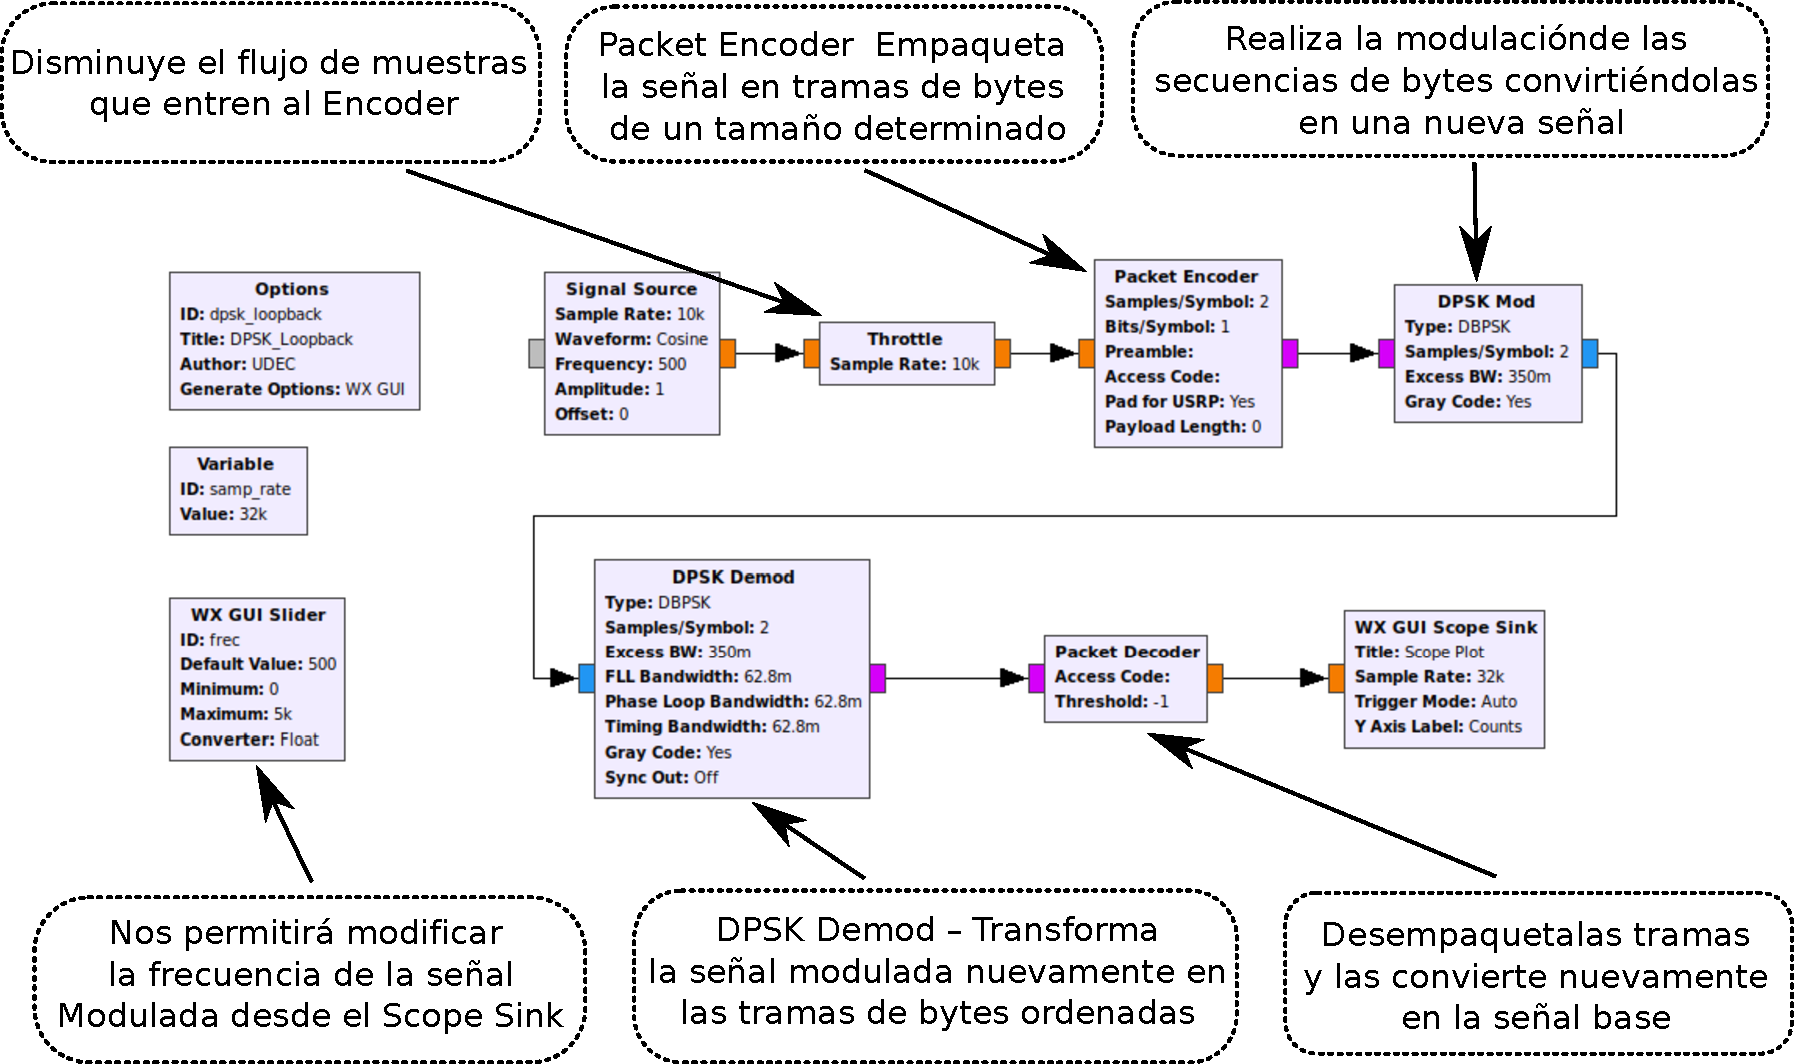
\includegraphics[width=0.9\textwidth]{Modulaciones_digitales/lab18/pdf/01Inicio.pdf}
\end{figure}
\end{frame}

	\begin{frame}
	\frametitle{\underline{\textbf{Objetivo de la guía del ejemplo Modulación DPSK}}}	
	Comprender el funcionamiento de los bloques de modulación y modulación DPSK, así como los bloques Packet Encoder y Packet decoder mediante la codificación y modulación de una señal, para luego recuperar la señal mediante la decodificación y modulación y finalmente ser vista en el ventana grafica WX GUI Scope Sink..\vspace{2mm}
	\end{frame}

	\begin{frame}
	\begin{enumerate}[1.]
	\frametitle{\underline{\textbf{Guía Ejemplo Modulación DPSK}}}
	\item{Modulador DPSK: En un modulador Dpsk, se realiza una operación XNOR entre el bit actual de la señal digital de información y bit transmitido con anterioridad. La salida de esta operación entra en un modulador PSK. En el modulador PSK, siempre que la salda de la puerta XNOR aparezca un 1 lógico, el modulador producira una salida analógica $+Cos(Wct)$. Si en lugar de esto la salida de la XNOR es un 0 lógico, en el modulador aparecerá la señal de salida $-Cos(Wct)$. Es decir, la salida de XNOR va a cambiar de valor cada vez que aparezca un 0 lógico en la señal digital de entrada al modulador, y por consiguiente producirá un cambio de fase analógica de salida.}\\

	\end{enumerate}
	\end{frame}	
	
	\begin{frame}
	\begin{enumerate}[1.]
	\frametitle{\underline{\textbf{Guía Ejemplo Modulación DPSK}}}
	\item{Demodulador DPSK: Es un circuito bastante simple que solo necesita un multiplicador analógico, un latch de retraso de 1 bit y un filtro pasa bajas con frecuencia de corte menor que $2Wc$. Cada vez que la salida del multiplicador es $Wct$, es decir se ha producido un cambio de fase entre la señal de entrada y señal anterior retrasada , a la salida del filtro pasa bajas aparece un 0 lógico, que es precisamente en lo que consiste la modulación DPSK. En caso contrario, si no se produce un cambio de fase la salida del filtro es un 1 lógico.}\\

	\end{enumerate}
	\end{frame}
	
	\begin{frame}
	\begin{enumerate}[1.]
	\frametitle{\underline{\textbf{Codificación y Modulación DPSK}}}
	\item{Packet Encoder: Empaqueta los bytes de una longitud y carga determinada con un encabezado, código de acceso y preámbulo.  El encabezado es un repetición 2x de la longitud de la carga útil (16 bits para cada campo).}\\
	\item{DPSK Mod este bloque modulador DPSK recibe en su entrada una secuencia de de bytes  (carácter sin signo) y en su salida entrega la señal modulada en banda base.}\\
	\end{enumerate}
	\end{frame}

\begin{frame}{Packet Encoder y DPSK Mod}
\begin{figure}[H]
	\vspace{-3mm}
	\centering
	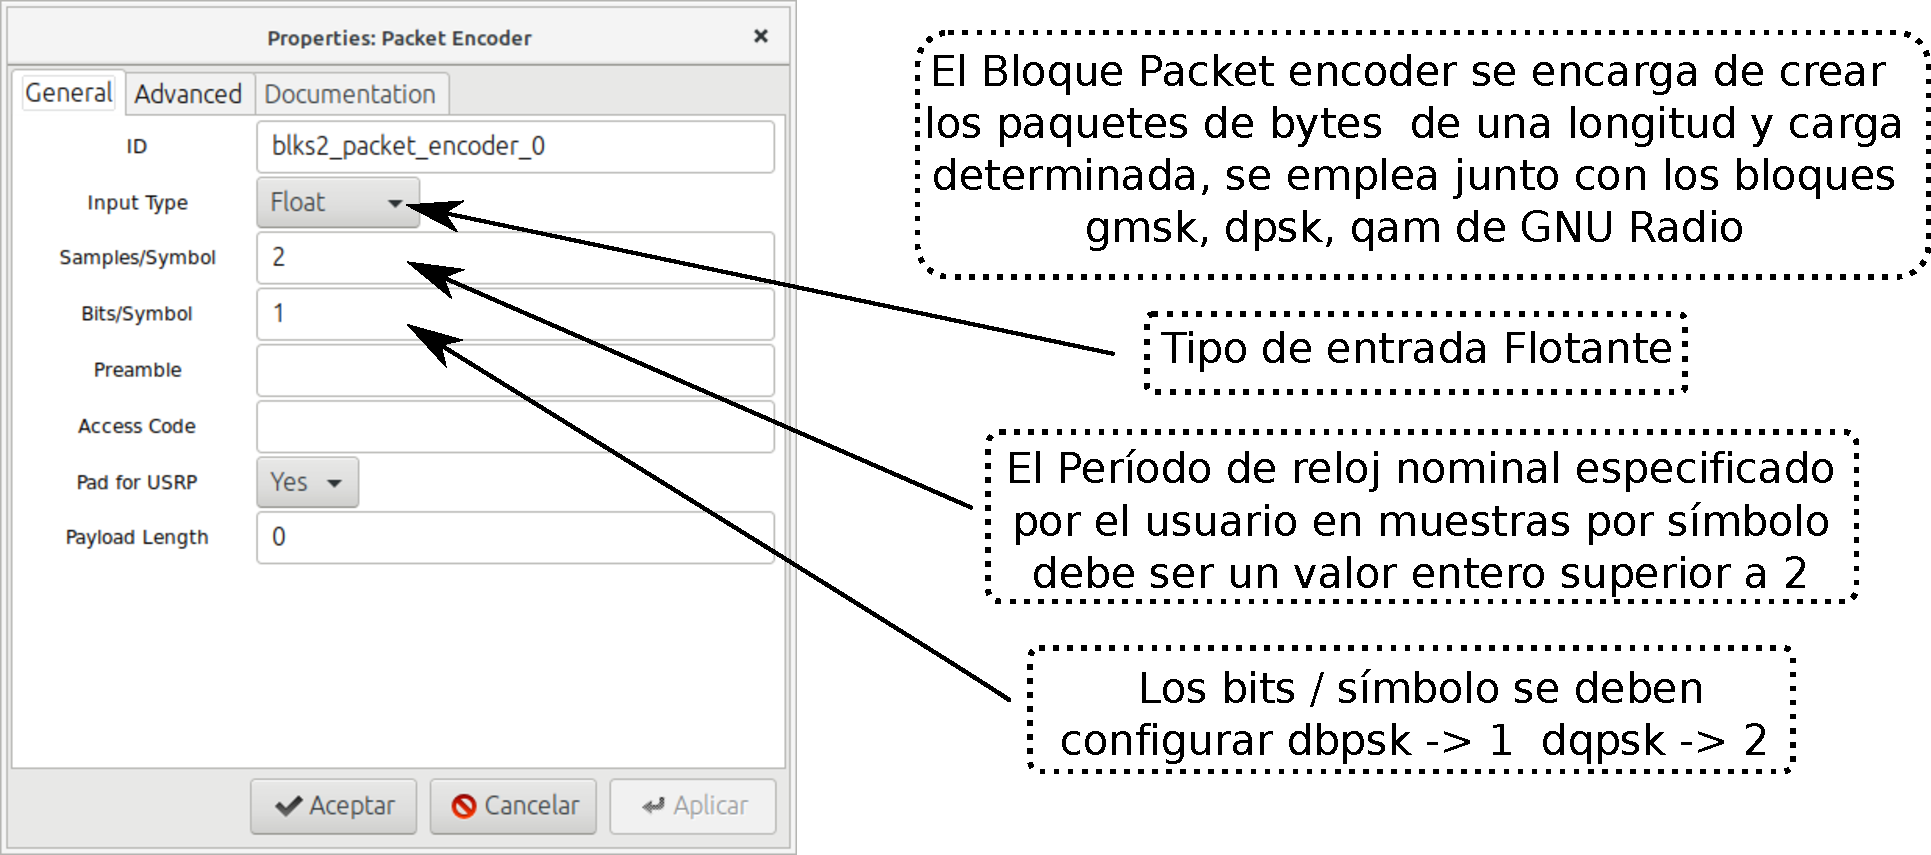
\includegraphics[width=0.9\textwidth]{Modulaciones_digitales/lab18/pdf/02Packet_Encoder.pdf}
\end{figure}
\end{frame}

\begin{frame}{Packet Encoder y DPSK Mod}
\begin{figure}[H]
	\vspace{-3mm}
	\centering
	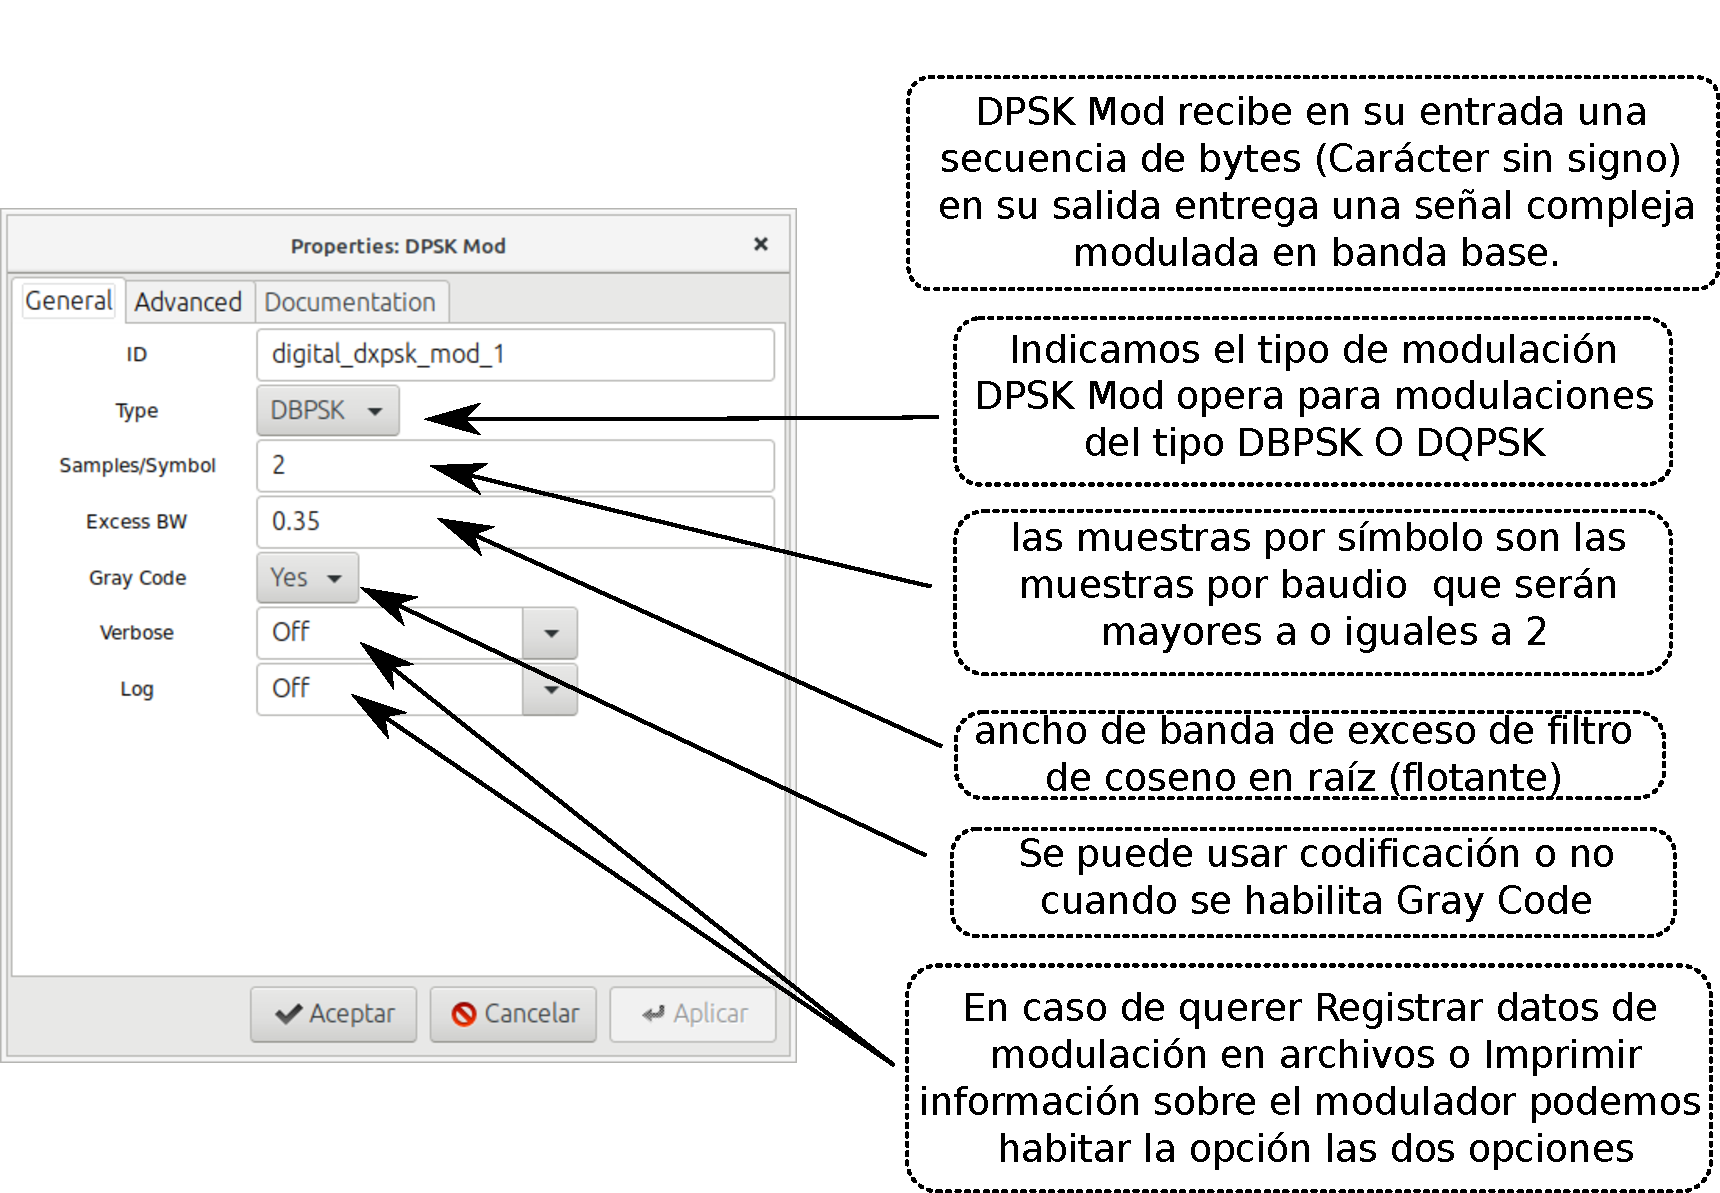
\includegraphics[width=0.9\textwidth]{Modulaciones_digitales/lab18/pdf/03DPSK_Mod.pdf}
\end{figure}
\end{frame}

	\begin{frame}
	\begin{enumerate}[1.]
	\frametitle{\underline{\textbf{Demodulación y Decodificación DPSK}}}
	\item{DPSK Demod: 
Realiza la demodulación de la señal compleja modulada en la frecuencia de banda base y entrega en su salida un flujo de bytes empaquetados }\\
	\item{Packet Decoder: El decodificador busca el código de  con el numero de bit disponibles incorrecto, cuando lo encuentra , lee el encabezado para obtener la longitud de la carga útil extraerla y generar la carga útil de bit original.}\\
	\end{enumerate}
	\end{frame}
	
\begin{frame}{DPSK Demod y Packet Decoder }
\begin{figure}[H]
	\vspace{-3mm}
	\centering
	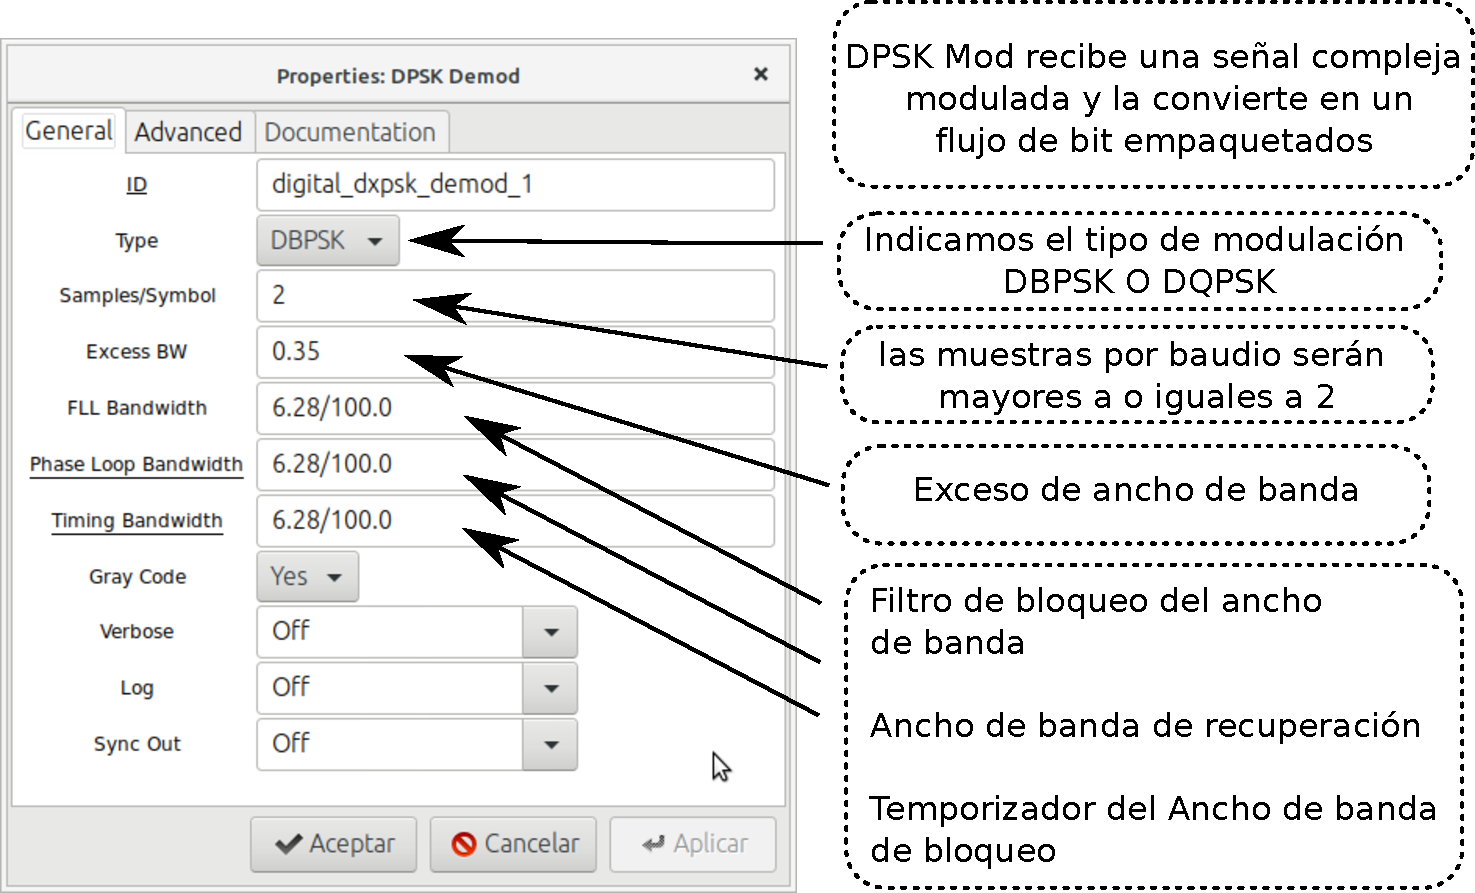
\includegraphics[width=0.9\textwidth]{Modulaciones_digitales/lab18/pdf/04DPSK_Demod.pdf}
\end{figure}
\end{frame}

\begin{frame}{DPSK Demod y Packet Decoder}
\begin{figure}[H]
	\vspace{-3mm}
	\centering
	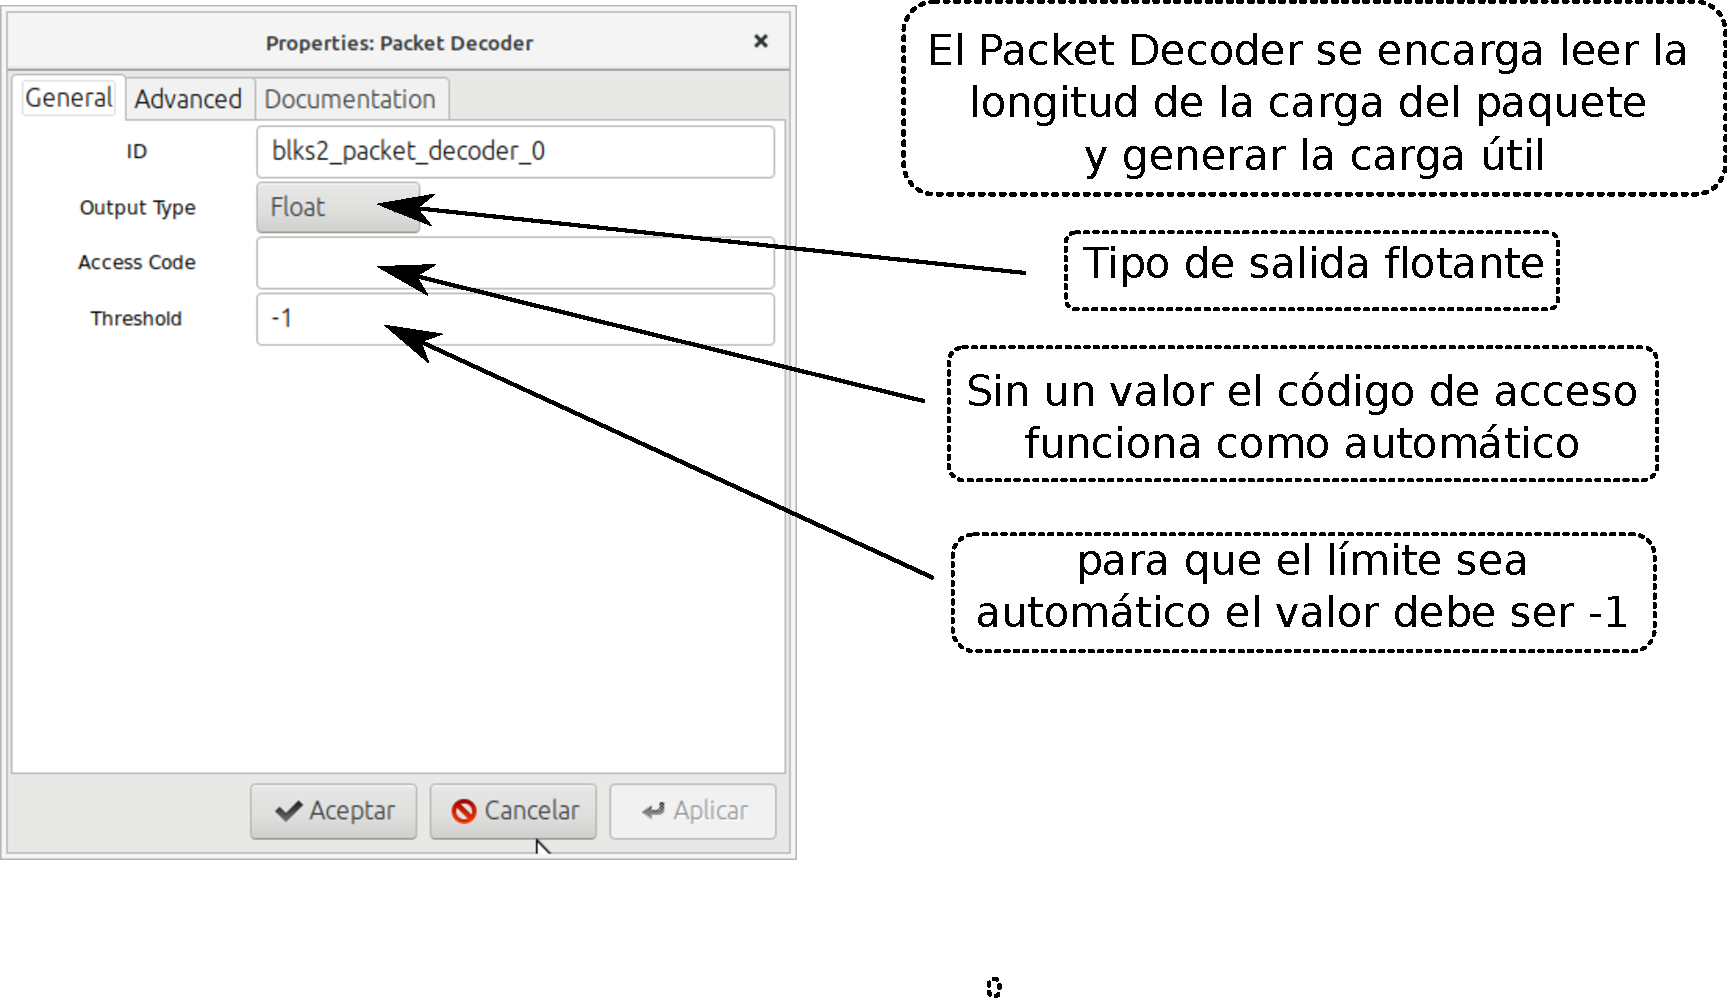
\includegraphics[width=0.9\textwidth]{Modulaciones_digitales/lab18/pdf/05Packet_Decoder.pdf}
\end{figure}
\end{frame}

\begin{frame}{ Señal Demodulada DPSK}
\begin{figure}[H]
	\vspace{-3mm}
	\centering
	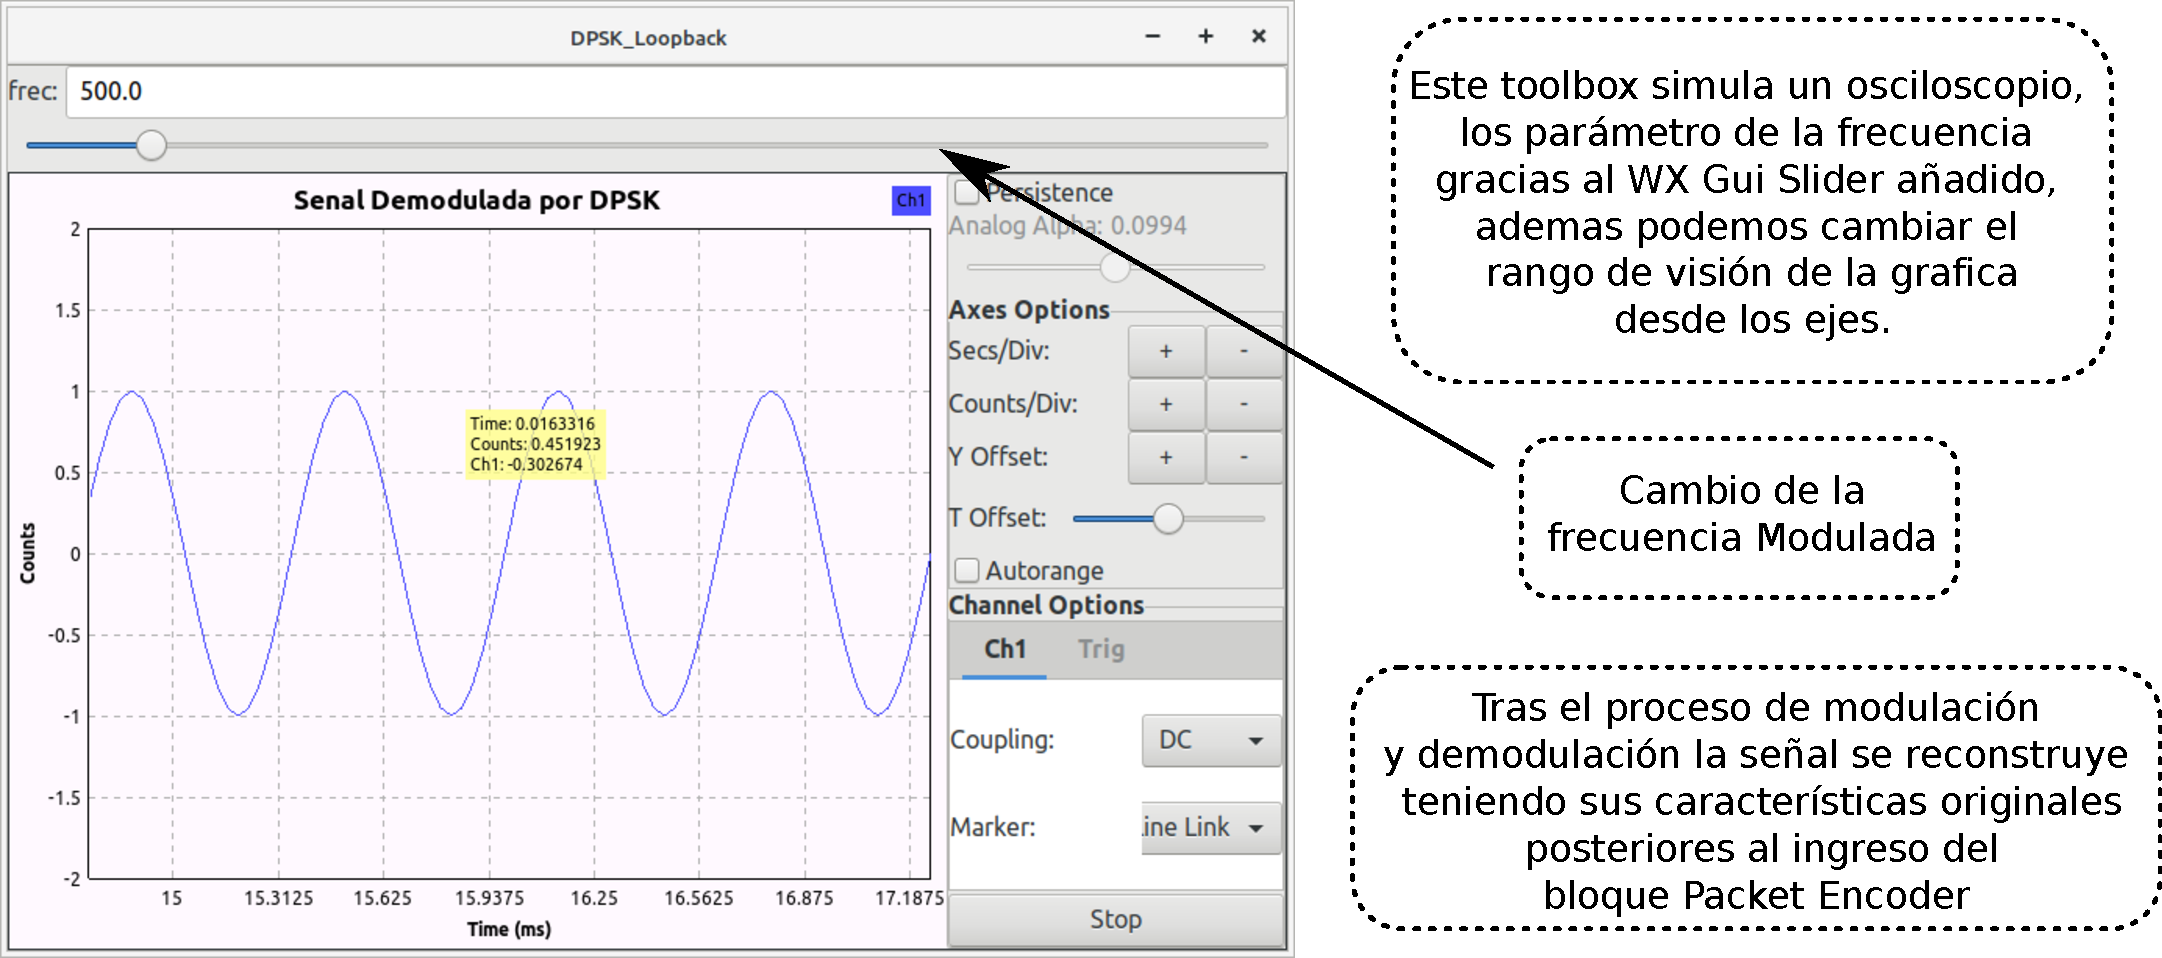
\includegraphics[width=0.9\textwidth]{Modulaciones_digitales/lab18/pdf/06Salida.pdf}
\end{figure}
\end{frame}
		


%\begin{frame}{Primeros pasos }
%\begin{figure}[H]
%	\vspace{-3mm}
%	\centering
%	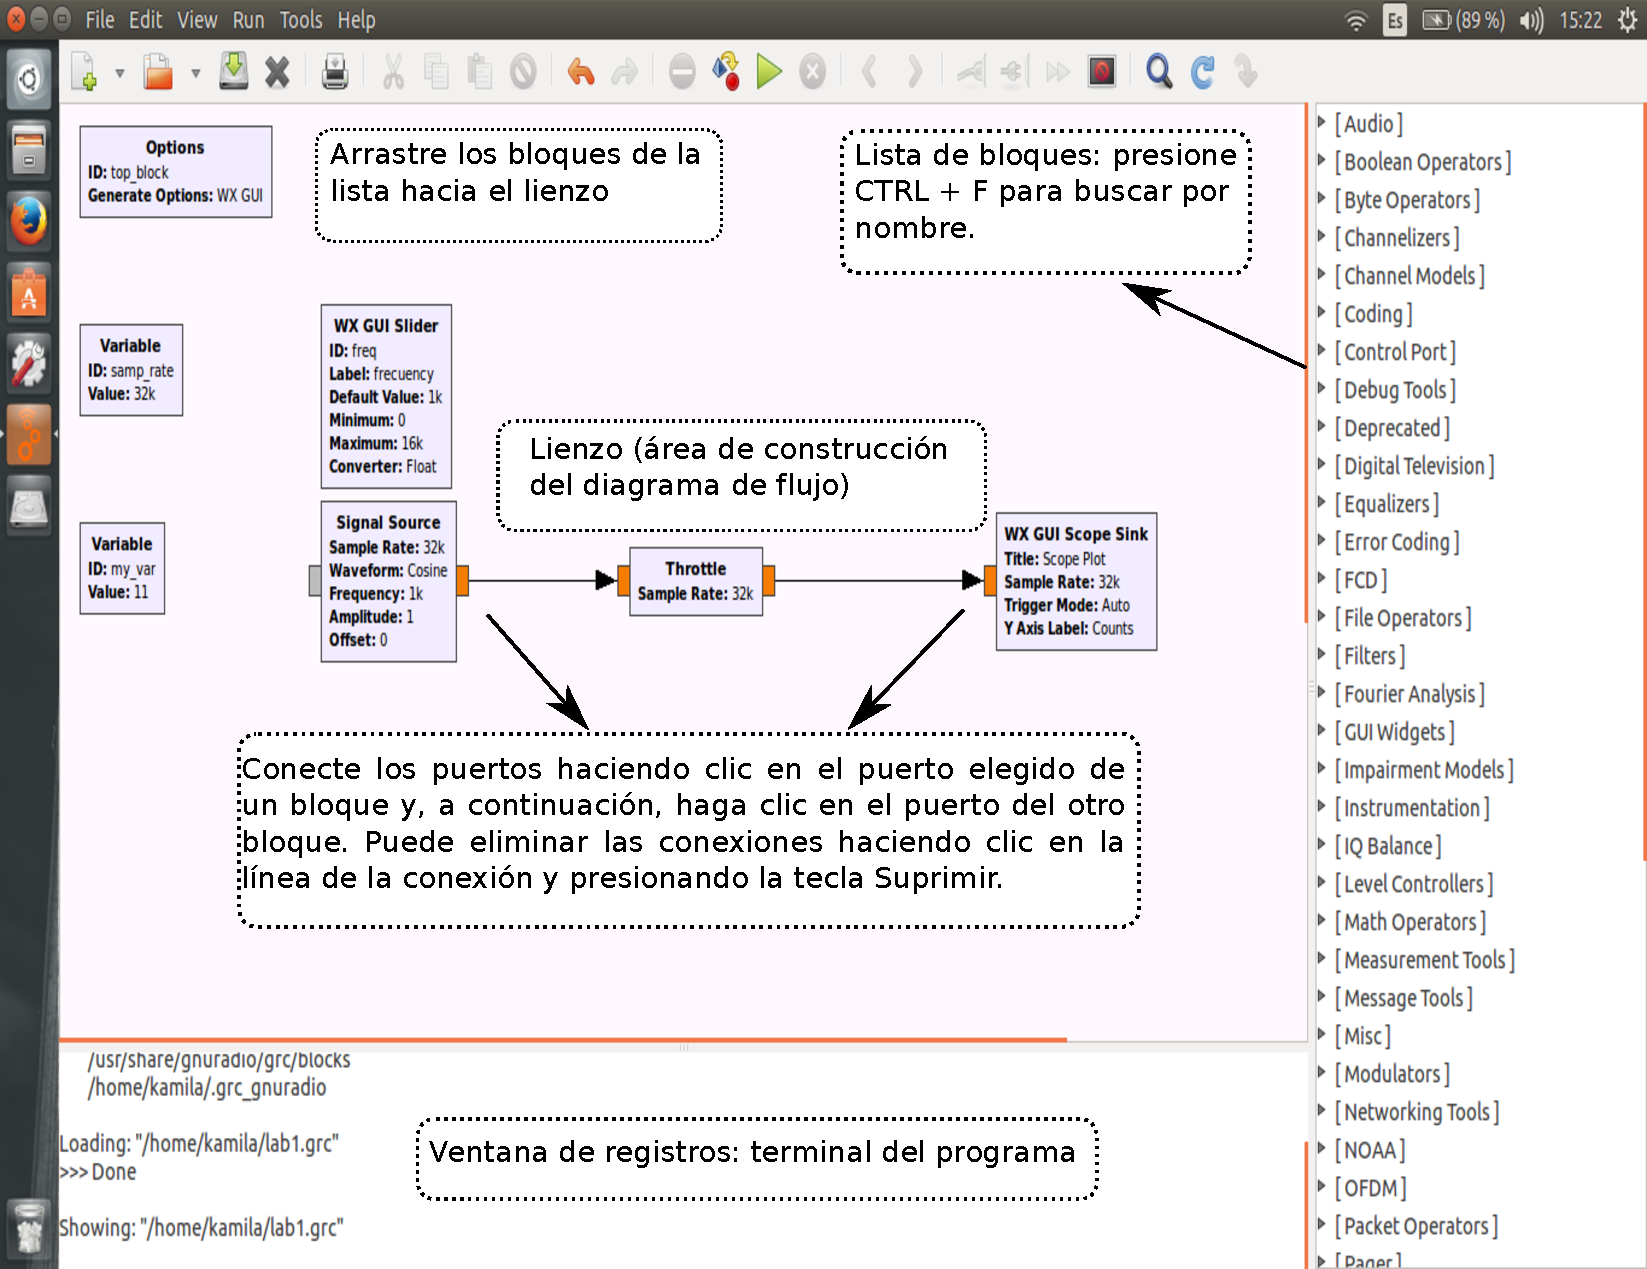
\includegraphics[width=0.9\textwidth]{Actividades2/pdf/lab1_1.pdf}
%\end{figure}
%\end{frame}